\section{Market Making}
\subsection{Что это такое}

Когда игрок приходит на биржу, он хочет купить актив по рыночной цене.
Если биржа $A$ продает биткоины по 11k\$, а биржа $B$ по 10k\$, то выгоднее покупать биткоины у $B$. Чтобы $A$ не терять клиентов, она пользуется услугами маркет-мейкеров.

Маркет-мейкеры решают проблему дисбаланса цен между биржами. Они могут за вознаграждение от биржи $A$ продать у них биткоины и выровнять курс до 10k\$, и тогда всем остальным будет снова выгодно торговать на бирже $A$. Аналогично работает, когда на бирже $A$ курс ниже относитьно других бирж: маркет-мейкеры закупятся биткоинами. В стабильное время маркет-мейкеры занимаются поддержанием маленького спреда, то есть делают так, что цены покупки и продажи отличаются как можно меньше.


\subsection{Как удерживают цену активов}

Маркет-мейкеры выставляют лимитные заявки на покупку/продажу на какой-то небольшой спред от индекс-цены. Обычно он равен комиссии биржи, это было выялвоено эмпирическим путем:

\begin{figure}[H]
\centering
\subfloat[Количество заявок на покупку/продажу]{
    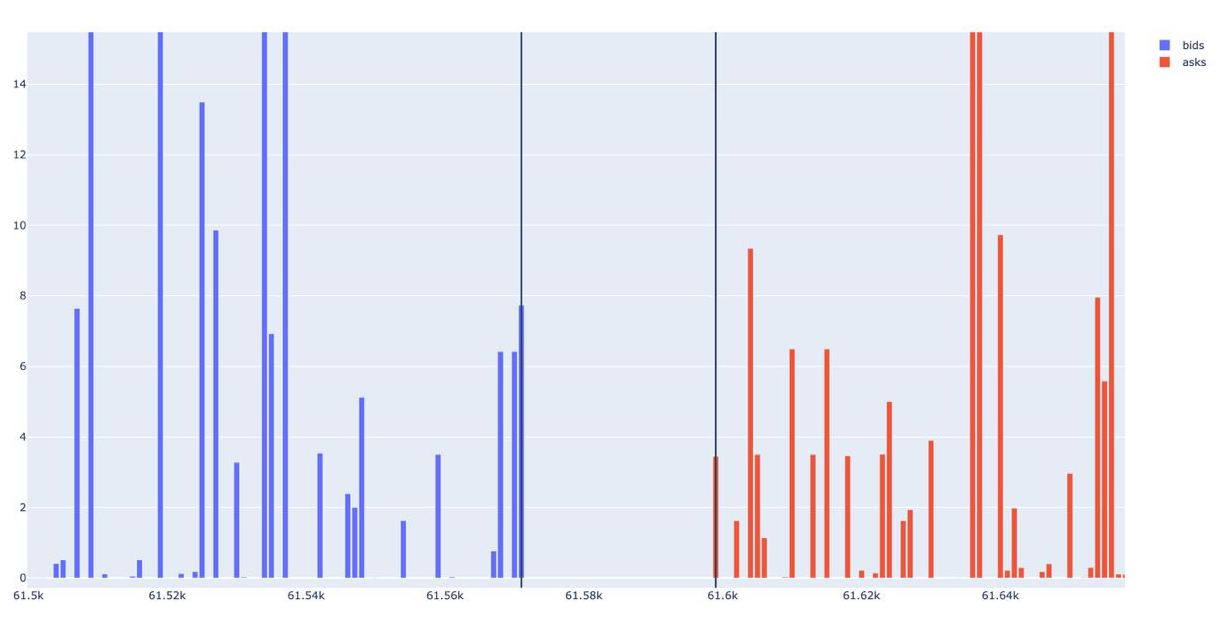
\includegraphics[width=0.9\linewidth]{img/bids_asks.png}
    }
\end{figure}

Черными вертикальными линиями отображены максимальная/минимальная цена, по которой выставлена лимитная заявка на покупку/продажу.

\definition \textbf{Спред} -- разница между максимальной/минимальной ценой лимитных заявкок на покупку/продажу.

Из наблюдений мы поняли, что спред чаще всего держится на уровне двух комиссий. Тем самамы маркет-мейкера дают пространство для торгов мелких игроков, которые просто пришли купить биткоин.

\subsection{Риски маркет-мейкинга}

\definition \textbf{Пробитием} будем называть ту заявку, которую мы не успели отменить, и по ней у нас открылась позиция.
\definition \textbf{Мейкер} -- тот, у кого исполнилась лимитная заявка на покупку/продажу.
\definition \textbf{Тейкер} -- тот, у кого исполнилась рыночная завка на покупку/продажу.
\remark Как правило, комиссия на бирже для мейкеров больше, чем для тейкеров. Свзяно это с тем, что если игрок исполняются заявку как мейкер, то  он сдвигает рыночную цену, и маркет-мейкерам нужно выставлять больше заявок для возвращения рынка в исходное положение.

Маркет-мейкерам нужен очень быстрый доступ в сеть и мощные вычислительные ресурсы, так как маркет-мейкер на бирже не один, и между ними есть конкуренция. В чем она заключается: если на какой-то бирже цена пошла резка вверх, то маркет-мейкерам нужно поддерживать спред уже по новой цене, соответсвенно, они будут отменять свои старые заявки и выставлять новые. В такой гонке те, кто не успевает за движеним рынка. Таких игроков пробивают, и им приходится исполнять мейкерски заявки, чтобы отыграть свое пробитие

\subsection{Как на этом можно заработать}

Заработать можно в предположении краткосрочно высоко-инерционного рынка.

Из-за того, что заявки, которые держат маркет-мейкеры на спреде, не бесконечны, то если придет крупный игрок, который моментально купит много актива, то есть столько, чтобы выкупить все, что держат маркет-мейкеры, то они не успеют переставлять свои заявки, и рынок отойдет от своего равновения. Однако из-за того, что это равновение было нарушено не каким-то рыночным фактором, а конкретным крупным игроком на конкретной бирже, то предпологается, что на этой бирже цена активов вернется в прежнее состояние. На этом предположении была построена следующая стратегия:

\begin{algorithm}
Market-Making orders
\begin{enumerate}

    \item \label{mm:init} Выставляем лимитные заявки в обе стороны на $\pm \Delta_1$ от индекс-цены.
    
    \item \label{mm:swap} Когда индекс-цена изменяется, переставляем заявки на ту же самую $\pm \Delta_1$, но уже от новой цены.
    
    \item Если переставиться успели, и нас не пробили, то переходим к шагу \ref{mm:swap}
    
    \item Неумаляя общности нас пробили на покупку по цене $p$. Отменяем все заявки
    
    \item Выставляем заявку на продажу на $\Delta_2$ от цены, по которой нас пробили на покупку
    
    \item \label{mm:win} Когда заявка исполнилась, возвращаемся к шагу \ref{mm:init}
    
\end{enumerate}
\end{algorithm}

В итоге на шаге \ref{mm:win} мы заработает $\Delta_2 \cdot p$.

\subsection{Реализация}
\href{https://github.com/dexety/dex-trading-system/tree/main/research/lp-0003-market-making}{Стратегия в репозитории}

Программа работает в трех потоках, которые нужны для: 

\begin{enumerate}

\item Выставление ордеров
\begin{enumerate}
    \item В этом потоке мы получаем новый трейды.
    \item Если цена нового трейда не такая, как у прошлого, и цена ордера, который надо выставить не такая, как у нас сейчас стоит, то мы отменяем текущие ордера и выставляем новые.
    \item Перестановка ордеров переходит не через сначала отмену, старых, а потом выставления новых ордеров, а непосредственно через переставление позиций аргументом \texttt{cancel\_id} в функции \texttt{create\_order}. Это позволило сократить количество запросов в два раза, а значит ошибка \texttt{Too many requests} будет встречаться реже.
\end{enumerate}

\item Получение обновлений ордербука
\begin{enumerate}
    \item В предыдущем потоке во время выставления и отмены ордеров новые обновления по вебсокету не приходят, но обновления ордер бука нам нужны, потому что по нему мы определяем цену оредров.
    \item Поэтому получения ордер бука вынесено в отдельный поток, чтобы всегда именть свежий стакан.
\end{enumerate}

\item Проверки положение ордеров
\begin{enumerate}
    \item Бывает так, что новые трейды не приходят, но окно спреда ордер бука меняется.
    \item Нам важно наше окно трейдов держать строго на $\pm$ какой-то спред вокруг бидсов и асков.
    \item Поэтому мы раз в какое-то время проверяем этот баланс, и если происходит дисбаланс, то мы обновляем наши ордера.
\end{enumerate}

\end{enumerate}

\subsection{Результаты}
Мы торговали на бирже \texttt{DyDx}. Она входит в топ самых популярных децентрализованных бирж. Количество сделок в месяц в ней около 30 тысяч и по биткоинку, и по эфиру. На самом деле это очень мало: в среднем 0.3 сделки в секунду, то есть одна сделка в 3-4 секунды. Соответственно рынок совсем не высоко-инерционный, и зачастую резкие скачки в цене связаны не с тем, что пришел крупный игрок и подвинул цену, а с тем, что на более курпных биржах сильно изменилась. Поэтому после того, как нас пробили в одну сторону, пробития во вторую не происходит.

Еще часто бывали случаи, когда рынок отскакивает в нужную нам сторону, но на величину меньше комиссии, соответственно, мы теряем деньги.

\subsection{Выводы}

Если бы у нас была нулевая или близка к нулевой комиссия, то мы бы были в плюсе. Но с той, что у нас есть, мы в минусе.
